\documentclass[a4paper]{dnd5}
\pagestyle{fancy}

\usepackage{wrapfig}

\newcommand\inc[1]{
 \includegraphics[width=0.22\textwidth, height=0.22\textwidth]{#1}
}

\newtoggle{DM}
\toggletrue{DM}
%\togglefalse{DM}

\begin{document}


\section*{Ships of the Northern Seas}

% http://www.british-towns.net/britain/history/ships

There are a number of basic ship designs in common use in the northern seas.  We cover a few here, but note that their exist a few experimental designs that include aspects of two or more of the designs below.

Warfare at sea is predominately a hand to hand affair.  Faster ships, having the weather gage and so on are all vitally important as they allow a ships captain to choose whether to enter combat at his advantage or to flee.  Black powder cannons are also fitted on some warships and some large trading vessels, though they are both inaccurate and unreliable when they hit the effects can be devastating.

 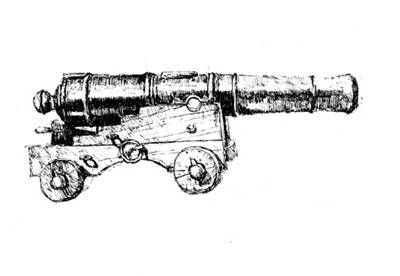
\includegraphics[width=0.22\textwidth]{ship_cannon.jpg}



\subsubsection*{Brythinian Holk}
\inc{brythynian_holk.jpg}

A holk is one of the technological predecessors of the carrack and caravel with a tonnage of 100 to 200 tons and 1 to 2 masts. The holk is peculiar to Brythinia where it is used primarily as a river or canal boat, with limited potential for coastal cruising.  More recently built holks have been developed that rival the cog as a major load carrier however the holk is being steadily replaced by the caravel.  Holks trade storage capacity for sea worthiness, having large cargo holds and weak frames (particularly at the bow and stern).

\subsubsection*{Caravel}
\inc{caravel.jpg}

A caravel is a small, highly maneuverable sailing ship with a tonnage of 50 to 160 tons, 1 to 3 masts, and lateen triangular sails giving her speed and the capacity for sailing to windward (beating). Caravels are much used by Averoignian and Brythinian merchants.

Being small and having a shallow keel, the caravel can sail upriver in shallow coastal waters. With the lateen sails attached, it is highly maneuverable and can sail much nearer the wind, while with the square sails attached, it is very fast. Its economy, speed, agility, and power make it esteemed as the best sailing vessel. The limited capacity for cargo and crew are its main drawbacks, but has not hindered its success.


\subsubsection*{Carrack}

\inc{carrack.jpg}

A carrack is a three- or four-masted sailing ship having a tonnage of between 90 and 220 tons.  Carracks were developed in Averoigne and are the preeminent large trading vessel in the northern seas. They have a high rounded stern with large aftcastle, forecastle and bowsprit at the stem and are usually square-rigged on the foremast and mainmast and lateen-rigged on the mizzenmast.

Carracks are ocean-going ships: large enough to be stable in heavy seas, and roomy enough to carry provisions for long voyages. 


\subsubsection*{Northern Cog}

\inc{northern_cog.jpg}

Cogs, though still widely used, are now somewhat out of date.  They are generally built of oak, are fitted with a single mast and a square-rigged single sail. These vessels are used for trading by Cheruskia and Hibernia. They are about 20 meters in length with a beam of about 6 meters.  The largest cog ships can carry up to about 130 tons.  Most cogs have open hulls and can be rowed short distances. The most recently built cogs now have decks.

The northern cog and the cheruskian warship are clinker built (using overlapping planks in the hull) all other ships in this document are carvel built (the planks butt up against one another).

Northern cogs differ significantly from those ships also called cogs in the middle seas and the two types are completely different types of ship.


\subsubsection*{Cheruskian Warship}
\inc{cheruskian_warship.jpg}

Cheruskian Warships are Cogs built to fight the Druchii on the open seas.  They have a forecastle and aftcastle making them less sea-worthy then their trading counter-parts.  They patrol the Boreal Sea in groups and engage the Druchii raiding galleys when they can with mixed results.  


\subsubsection*{Druchii Galley}
\inc{dark_elf_galley.jpg}

The Druchii Galley is a type of ship that is propelled mainly by rowing. The galley is characterized by its long, slender hull, shallow draft and low clearance between sea and railing.  It can be fitted with lateen sails in favourable winds, but human strength is always the primary method of propulsion. This allows galleys freedom to move independently of winds and currents, and with great precision. 

The Druchi primarily use the galleys to plunder coastal communities and for marauding trading ships.  They use slaves to man the oars.  It is said that the number of these ships that have is vast and limited only by their ability to source good timber for the creation of more.


\subsubsection*{Hibernian Buss}
\inc{hibernian_buss.jpg}

A buss is a type of seagoing fishing vessel, originally used as a cargo vessel but now adapted for use by Hibernian herring fishermen as a fishing vessel after the invention of gibbing made it possible to preserve herring at sea (a process of selective removal of organs and salting, circa 2030 AUC).  This made longer voyages feasible, and hence enabled Hibernian fishermen to follow the herring shoals far from the coasts. 

These ships are about 20 meters in length, displace between 60 and 100 tons, and have a round-bilged keel and a round bow and stern, the latter relatively high, and with a gallery. The broad deck provides space to process the catch on board.  They are a relatively nimble ship, though still sufficiently stable to be seaworthy.

The ship has two or three masts. The mainmast and foremast (if present) can be lowered during fishing, leaving only the mizzen mast upright. It is square rigged on the main mast, with a gaff rig on the mizzen and has a long bow sprit with jibboom and up to three headsails.

The ships sail in large fleets of 400 to 500 ships to the fishing grounds around Albion and the Orkides isles. They are usually escorted by naval vessels, because Druchii raiding parties are common in the area.  These fleets stay at sea for weeks at a time. Their catches would sometimes be brought home by special ships (called ventjagers) while the fleet would still be at sea.  

The busses use long drift nets to catch the herring. Such nets hang like curtains across the travel paths of the herring schools.  The nets would be taken aboard at night and then the crews of eighteen to thirty men would start the gibbing, salting and barrelling immediately.

There are three to four voyages per season (depending on the weather and the catch). In the off-season the busses are used as normal cargo vessels, for instance to transport grain from Cheruskia, or salt from the Wild Coast. 


\subsubsection*{Hoy (or Cromster)}
\inc{hoy.jpg}

The Hoy or Cromster is a type of small warship used by the Hibernians and Brythinian fleets.  It is designed for work inshore on the shoal coasts and is a ketch, spritsail rigged on the main, and lateen on the small mizzen, usually displacing about 60 tons.  For its size, it is heavily armed.

A combination of manoeuvrability, shallow draught, and heavy artillery make the Hoy one of the most effective warships in coastal waters.  
\end{document}
